\chapter{Background Theory}
\label{ch:background}

This section briefly introduce fundamental technologies that current research based on. Section \ref{sec:bg_aam} explains the manner of constructing statistical deformable models using active appearance model. Section \ref{sec:bg_icp} briefly described the mechanical of Iterative Closest Points and the reason of using ICP for pre-processing. Section \ref{sec:bg_svs} introduces a shape discriminator which is infinitely differentiable. Section \ref{sec:bg_opticalflow} brings the technologies of registering video sequences. Our research takes the idea from optical flow in order to put shapes in dense correspondence. Section \ref{sec:SSD} presents the algorithm of steepest descend for minimising error function when fitting objects.

\section{Active Appearance Model (AAM)}
\label{sec:bg_aam}
An Active Appearance Model (AAM) is a combination of linear statistical shape and appearance model with corresponding fitting algorithms \cite{Matthews2004, Cootes2001}. AAM separate that model in two parts, shape model and appearance model. 

\subsection{Shape Model}
Shapes are defined as vertexes of a mesh. A shape model is a function that can express arbitrary shapes by using a base shape plus a linear combination of shape vectors. Mathematical definition of shape model shown below:
\begin{equation}
s=s_0+\sum^n_{i=1}p_i s_i
\end{equation}
where shape $s$ is expressed by base shape $s_0$ plus linear combination of shape vectors $s_i$, each having coefficient $p_i$. Note that $s_i$ need to be orthonormal. In general, shape model are generated by applying Principle Component Analysis (PCA). Therefore $s_0$ is the mean shape with $s_i$ are eigenvectors(principle components).

\subsection{Appearance Model}
\label{sec:appearance_model}
Appearances are defined as pixels lie inside base shape $s0$. Similar to shape models, appearance models are defined in same format, a base appearance plus linear combination of appearance vectors. Mathematical definition of appearance model is expressed below:
\begin{equation}
A(x)=A_0(x)+\sum^m_{i=1}\lambda_iA_i(x)
\end{equation}
where $x \in s0$, appearance $A(x)$ is expressed by base appearance $A_0(x)$ plus linear combination of appearance vectors $A_i(x)$, each having coefficient $\lambda_i$. Note that $A_i(x)$ need to be orthonormal. In general, appearance model are generated by applying Principle Component Analysis (PCA). Therefore $A_0(x)$ is the mean appearance with $A_i(x)$ are eigenvectors(principle components).

\subsection{AAM Instance}
Active Appearance Model combines shape model and appearance model to generate instances. Instance generating procedure is starting with compute warping from base shape $s_0$ to instance shape $s$, to be more specific, piecewise affine warp in general. The warp is required to map appearance instance $A(x)$ to shape instance $s$ since appearance instance is built on base shape $s_0$. The way piecewise affine works is finding corresponding triangles in both base shape and instance shape, then for each pixels within a triangle on $s_0$, finding position of the pixel of same triangle in $s$. The final model instance should satisfies  following expression:
\begin{equation}
M(W(x;p))=A(x)
\end{equation}
where $M$ is AAM instance and $W(x;p)$ represent piecewise affine warp.

\subsection{AAM Fitting}
In the case of fitting an AAM to an input image $I(x)$, aam instance $M(W(x;p))=A(x)$ should be similar as $I(x)$. For any pixel $x$ in base shape $s_0$, the corresponding pixel in the input image is $W(x;p)$. Appearance of pixel $x$ are defined as $A(x)=A_0(x)+\sum^m_{i=1}\lambda_iA_i(x)$ mentioned in section \ref{sec:appearance_model}. For pixel $W(x;p)$, appearance of input image is expressed as $I(W(x;p))$. A formal fitting algorithm can now be defined: the objective is to discover optimal AAM instance that fit given input image maximumly. In other words, we want to minimise following error function to minimise difference between $A(x)$ and $I(W(x;p))$:
\begin{equation} 
\label{eq:aamfittingbase}
E(x)=||A_0(x)+\sum^m_{i=1}\lambda_iA_i(x)-I(W(x;p))||^2
\end{equation}
where input image is denoted as $I$ and $||.||^2$ is the L2 norms. To be more specific, image $I$ is warped back onto base shape $s_0$ before computing difference against AAM instance appearance.

\subsection{Alternating Minimisation}
As the expression revealed, there are two variables contained ($p$ and $\lambda$) so it is of importance to minimise them simultaneously. As there is no dependency between AAM shape and appearance, solving $p$ and $\lambda$ alternatively is plausible. Considering creating a linear subspace, which is spanned by collection of appearance component vector $A_i$, denoted as $span(A_i)$ and $span(A_i)^\perp$ as orthogonal complement subspace. Therefore \ref{eq:aamfittingbase} can be rewrite as:
\begin{equation} 
\label{eq:aamfittingappearancevariance}
E(x)=||A_0(x)+\sum^m_{i=1}\lambda_iA_i(x)-I(W(x;p))||^2_{span(A_i)^\perp}+||A_0(x)+\sum^m_{i=1}\lambda_iA_i(x)-I(W(x;p))||^2_{span(A_i)}
\end{equation}
where $||.||^2_L$ is L2 norm of vector projected into linear subspace $L$. Because norm considers only orthogonal components of subspace $L$ so any components lies in $L$ can be dropped. So the above function can be optimised as:
\begin{equation} 
\label{eq:aamfittingappearancevariancesubspace}
E(x)=||A_0(x)-I(W(x;p))||^2_{span(A_i)^\perp}+||A_0(x)+\sum^m_{i=1}\lambda_iA_i(x)-I(W(x;p))||^2_{span(A_i)}
\end{equation}
The first section contains only variable $p$, therefore the optimal value of the equation can be found by first minimising $||A_0(x)-I(W(x;p))||^2_{span(A_i)^\perp}$ with respect to $p$ alone before substitute minimal $p$ value in $||A_0(x)+\sum^m_{i=1}\lambda_iA_i(x)-I(W(x;p))||^2_{span(A_i)}$ then minimise with respect to $\lambda$. Mathematical equations shown below:
\begin{equation}
\label{eq:minimisep}
\operatorname*{arg\,min}_p=||A_0(x)-I(W(x;p))||^2_{span(A_i)^\perp}
\end{equation}
Based on the assumption of basis vector $A_i$ are orthonormal, $\lambda$ can be computed with closed-form solution:
\begin{equation}
\label{eq:minimiselambda}
\lambda_i=\sum_{x\in s_0}A_i(x).[I(W(x;p))-A_0(x)]
\end{equation}

\subsection{Image Alignment}
Minimising equation \ref{eq:minimisep} also referenced as Image Alignment. The purpose of image alignment is finding constant template image in given input image \cite{Matthews2004}. 

\subsubsection{Lucas-Kanada Algorithm}
Using gradient descent method for image alignment was first introduced by Lucas Kanada by minimising square error between two images which having same form as equation \ref{eq:minimisep}. Solving $p$ is a nonlinear process as pixel value of an image generally unrelated to pixel coordinate. Lucas Kanada make the problem linear by solving the problem with an incremental parameter $\delta p$ with assumption that initial value of $p$ is known. Thus the problem can be solved iteratively for $\delta p$. Equation \ref{eq:minimisep} can now be solved with respect to $\delta p$ as:
\begin{equation}
\label{eq:minimisedp}
||A_0(x)-I(W(x;p+\delta p))||^2
\end{equation}
where $p$ gets updated at every iteration by $p=p+\delta p$. A Taylor expansion on above function gives:
\begin{equation}
\label{eq:minimisedptaylor}
||A_0(x)-I(W(x;p))-\nabla I\frac{\partial W}{\partial p} \delta p))||^2
\end{equation}
where $\frac{\partial W}{\partial p}$ is the Jacobian and $\nabla I$ is image gradient. $\delta p$ can be solved in closed form:
\begin{equation}
\label{eq:dp}
\delta p=\bm{H}^{-1}\sum_x[\nabla I\frac{\partial W}{\partial p}]^T[A_0(x)-I(W(x;p))]
\end{equation}
where $\bm{H}$ is the Hessian matrix:
\begin{equation}
\label{eq:hessian}
\bm{H}=\sum_x[\nabla I\frac{\partial W}{\partial p}]^T[\nabla I\frac{\partial W}{\partial p}]
\end{equation}
The new variable $p$ can now be updated by $p=p+\delta p$ before involving in next iteration of optimisation. Iterations ends when converged or specific criteria reached. 

However, Lucas-Kanada Gaussian-Newton descent is slow due to computational intensity on Hessian Matrix $\bm{H}$, which contains image gradient $\nabla I$ and warp Jacobian $\frac{\partial W}{\partial p}$ and both depends on $p$ but $p$ is varying at every iteration. Besides, computation of $\nabla I$ $\frac{\partial W}{\partial p}$ also slow.

\subsubsection{Forwards Compositional Algorithm}
\label{sec:fca}
Instead of updating $p$ from estimated $\delta p$ iteratively, \cite{Matthews2004} mentioned compositional algorithms of updating warp transformation. The cost function are:
\begin{equation}
\label{eq:forwardcomposition}
||A_0(x)-I(W(W(x;\delta p);p))||^2
\end{equation}
where $W(x;\delta p)$ denotes incremental warp. The update step of new warp $W(x;p)$ is:
\begin{equation}
W(x;p) = W(x;p)\circ W(x;\delta p)
\end{equation}
Applying Taylor expansion on equation \ref{eq:forwardcomposition} gives:
\begin{equation}
\label{eq:forwardcompositiontaylor}
||A_0(x)-I(W(W(x;0);p))-\nabla I(W(x;p))\frac{\partial W}{\partial p}\delta p||^2
\end{equation}
where $W(x;0)$ is the identical warp that $W(x;0) = x$. Comparing with equation \ref{eq:minimisedptaylor}, image gradient is now computed for $I(W(x;p))$. The key improvement is that update of warp is evaluation with respect to $p=0$ therefore Jacobian is now computed at $(x;0)$. Thus a constant Jacobian through all iterations so can be precomputed.

\subsubsection{Inverse Compositional Algorithm}
Inverse Compositional Algorithm are based on Forwards Compositional Algorithm that the purpose of template image $A_0(x)$ and input image $I$ are inversed to further improve performance by precomputing $\delta p$ and Hessian matrix \cite{Matthews2004}. Cost function for inverse compositional algorithm are:
\begin{equation}
\label{eq:inversecomposition}
||I(W(x;p))-A_0(W(x;\delta p))||^2
\end{equation}
where $W(x;\delta p)$ denotes incremental warp on template image. So the update step of new warp $W(x;p)$ is:
\begin{equation}
W(x;p) = W(x;p)\circ W(x;\delta p)^{-1}
\end{equation}
Applying Taylor expansion on equation \ref{eq:inversecomposition} gives:
\begin{equation}
\label{eq:inversecompositiontaylor}
||I(W(x;p))-A_0(W(x;\delta p))-\nabla A_0\frac{\partial W}{\partial p}\delta p||^2
\end{equation}
where $W(x;0)$ is the identical warp that $W(x;0) = x$. The closed form solution of $\delta p$ is:
\begin{equation}
\label{eq:dpic}
\delta p=\bm{H}^{-1}\sum_x[\nabla A_0\frac{\partial W}{\partial p}]^T[I(W(x;p))-A_0(x)]
\end{equation}
where $\bm{H}$ is the Hessian matrix:
\begin{equation}
\label{eq:hessianic}
\bm{H}=\sum_x[\nabla A_0\frac{\partial W}{\partial p}]^T[\nabla A_0\frac{\partial W}{\partial p}]
\end{equation}
As the equation states, image template $A_0$ is constant and $\frac{\partial W}{\partial p}$ is evaluated at $p=0$ same as the Jacobian part in forward compositional algorithm. Therefore both $\delta p$ and Hessian $\bm{H}$ can be precomputed before optimising cost function. 

\subsection{Pseudo Algorithms}

The pseudo code of AAM fitting using inverse compositional algorithm is shown in Algorithm \ref{alg:aam}\cite{Matthews2004}:

\begin{algorithm}[ht]
\caption{Fitting Active Appearance Model with Inverse Compositional Algorithm}
\label{alg:aam}
Compute gradient $\nabla A_0$ of image template $A_0(x)$\;
Compute Jacobian $\frac{\partial W}{\partial p}$ at $(x;0)$\;
Compute Hessian matrix $H$\;
\While{not converged or criteria not met}{
    Warp input image $I$ with transform $W(x;p)$\;
    Compute error image $I(W(x;p))-A_0(x)$\;
    Compute $\delta p$ by multiplying inverse Hessian matrix $H^{-1}$\;
    Update warp by $W(x;p) = W(x;p)\circ W(x;\delta p)^{-1}$\;
    Update $\lambda$ by $\lambda_i=\sum_{x\in s_0}A_i(x).[I(W(x;p))-A_0(x)]$\;
}  
\end{algorithm}


% AAM is trained using a set of images where each image contains clear annotated images using same number of landmarks. Shape model is trained using landmark coordinates before applying PCA on shapes to produce a mean shape with some eigenvectors to control the deformation of mean shape. For training appearance model, training images are warped to a reference frame, which contains landmarks of mean shape, so we have different objects with same shape but different texture. Then PCA is used again applying on the warped images to generate mean appearance with eigenvectors controlling variations of texture. Fitting an AAM model to a new image is using Lucas Kanade Alternating Inverse Composition algorithm which is clearly explained in references \cite{Matthews}.
\section{ICP \& NICP}
\label{sec:bg_icp}
\subsection{Iterative Closest Point}
Iterative Closest Point (ICP) is an algorithm for aligning two different point clouds\cite{Besl1992}. In the situation of aligning point cloud A to point cloud B (named source and target correspondingly), the algorithm finds the transformation matrix that best matches source to target. The procedure can be briefly summarised as following steps:
\begin{itemize}
  \item For each point in source, finding corresponding closest point in target.
  \item Calculating optimal rotation, translation and scaling transform to minimise difference (measured in point-to-point mean square error) between source and points generated in previous step.
  \item Transform source using translation calculated in previous step to obtain new source.
  \item Iterate until converge or special criteria satisfied.
\end{itemize}
\cite{Besl1992} shows ICP convergence can be proved that it will always converge to a local minimum.

\subsection{Non-rigid Iterative Closest Point}
Although ICP provided notable solution of aligning point clouds, it provides only rigid alignment that finding the best affine transform between source and target. For objects e.g. faces, ears, human poses, bottles and objects that are highly deformable, ICP is weak at model local changes and produces biased result due to non-rigid deformation.

Non-rigid Iterative Closest Point (NICP) are an extension of ICP having enabling source to deform to fit target without breaking the property of guaranteed convergence\cite{Amberg2007}. A new term stiffness is introduced in order to constrain the degree of deformation. The fundamental idea is to incrementally apply ICP with stiffness where stiffness are scaling from high to low value at each iteration. To be specific, at initial iteration, the algorithm turned to apply rigid ICP on source, but source are allowed to deform in later iteration with increasingly extent. After converging, each point of source have one-to-one correspondence of points on target.

In the situation of registering source $S$ to template $T$, $S$ are defined as mesh $(V,E)$ where $V$ are vertices and $E$ are edges with corresponding amount $n, m$. Template $T$ can have vertices only without defining edges. Registering $S$ to $T$ means computing a transformation matrix $X$ so that $V(X)$ is the projection of each points on target. Proper definition of $X$ are:
\begin{equation}
\label{eq:nicpX}
X=[X_1,X_2,\dotsc,X_n]^T
\end{equation}
where $X_i$ is affine $3\times 4$ transformation matrix so $X$ are $4n\time 3$ matrix. The comprehensive cost function of optimising $X$ are:
\begin{equation}
E(X)=E_d(X)+\alpha E_s(X)+\beta E_l(X)
\end{equation}
where $E_d(X)$ is distance penalty term, $E_s(X)$ is stiffness penalty term and $E_l(X)$ is landmark penalty term. Definitions of each term are detailedly introduced in following sections \ref{sec:nicpdt}, \ref{sec:nicpst} and \ref{sec:nicplt}.

\subsubsection{Distance Penalty Term}
\label{sec:nicpdt}

Distance between $S$ and $T$ are defined using Euclidean Distance. The distance penalty term and corresponding matrix form is defined as~\cite{Amberg2007}:

\begin{align}
\label{eq:nicpdt}
E_d(X) &= \sum_{i=1}^n{w_i || X_i v_i - u_i ||^2} 
\\ &=
\begin{Vmatrix}
    (W \otimes I_3) 
    \begin{pmatrix}
        \begin{bmatrix}
        X_1 &  &  \\  & \ddots &  \\ &  & X_n
        \end{bmatrix}
        \begin{bmatrix}
        v_1 \\ \vdots \\ v_n
        \end{bmatrix}
        -
        \begin{bmatrix}
        u_1 \\ \vdots \\ u_n
        \end{bmatrix}
    \end{pmatrix}
\end{Vmatrix}
^2
\end{align}

where $v_i \in V$ are assumed having format $[x,y,z,1]^T$, $u_i \in T$ is corresponding closest point with same format of $v_i$, Euclidean distance between $v_i$ and $u_i$ is weighted by $w_i$. For matrix form, $W$ has form $\text{trace}(w_1,...,w_n)$ and performs Kronecker tensor product with an identity matrix of shape $3 \times 3$. 

By defining $D = \text{trace}(v_1,\dotsc,v_n)$ and $U=[u_1,\dotsc,u_n]^T$, above equation can be further simplified as:
\begin{equation}
E_d(X) = ||W(DX-U)||^2_F
\end{equation}

\subsubsection{Stiffness Penalty Term}
\label{sec:nicpst}

Stiffness term is introduced to have constrain on deformation. In other word, stiffness maintains the neighbouring  correlation for each vertex. A significant deformation of one vertex can cause remarkable penalty on neighbouring vertices. Therefore source mesh cannot deform completely freely but with regularisation. The matrix form of stiffness penalty cost function defined as~\cite{Amberg2007}:
\begin{equation}
E_s(X)=||(M \otimes G)X||^2_F
\end{equation}
where $M$ expresses the connectivity of vertices with $m \times n$ that each row $r$ represent an edge, for edge connecting vertices $(i,j)$, $M_{ri}=-1$ and $M_{rj}=1$. $G=\text{trace}(1,1,1,\gamma)$, where $\gamma$ used to weight skew and rotation part of deformation.

\subsubsection{Landmark Penalty Term}
\label{sec:nicplt}

Landmark penalty term functioning similar as distance term. It can be assumed as a sparse version of distance term with exact landmark correspondence instead of looking up for closest points. Formal definition are~\cite{Amberg2007}:
\begin{equation}
E_l(X)=||D_LX-U_L||^2_F
\end{equation}
where $D_L$ are rows from matrix $D$ that related to landmark points and similarly $U_L$ are of format $[l_1,\dotsc,l_l]^T$ with $l_i$ as landmark points.

\cite{Amberg2007} shown landmarks term is optional. Although landmark term accelerated converge rate, NICP still produced desirable result without this term.

\subsubsection{Comprehensive Cost Function}
As each of penalty terms are defined in details above, the finalised cost function can be expressed:
\begin{align}
\label{eq:nicpfinal}
E(X) &= 
\begin{Vmatrix}
    \begin{bmatrix}
        \alpha M \otimes G \\ WD \\ \beta D_L
    \end{bmatrix}
    X- 
    \begin{bmatrix}
        0 \\ WU \\ U_L
    \end{bmatrix}
\end{Vmatrix}
^2_F \\
&= ||AX-B||^2_F,
\end{align}
where $X$ can be solved directly by setting the derivative of $E(X)$ to zero. So $X$ has a closed-form solution:
\begin{equation}
\label{eq:nicpx}
X=(A^TA)^{-1}A^TB
\end{equation}
which simply is the product of pseudo-inverse of matrix $A$ and matrix $B$. Therefore in each step, the deformation can be found directly for fixed $\alpha$ and $\beta$. Since landmark term is optional, the final algorithm considers only varying stiffness weighting. Pseudo code are shown below~\cite{Amberg2007}:
\begin{algorithm}[ht]
\caption{Non-rigid Iterative Closest Point Algorithm}
\label{alg:nicp}
Initialise $X^0$ as identical transformation\;
\For{$\alpha \in [\alpha^1,\dotsc,\alpha^p] \& \alpha_i > \alpha_{i+1}$}{
    \While{$||X^j-X^{j-1}||^2_F > \varepsilon$}{
        Calculate new source $S=(V(X^{j-1}),E)$\;
        Find optimal $X^j$ between $S$ and $T$ using equation \ref{eq:nicpx}\;
    }
}
Return $X$\;
\end{algorithm}

As Nonrigid ICP declared that it preserved convergence feature from ICP so the algorithm \ref{alg:nicp} also gauranteed termination. Detailed discussion convergence preservation can be found in~\cite{Amberg2007}.
\section{Support Vector Shape (SVS)}
\label{sec:bg_svs}
Support Vector Shape (SVS) introduces an implicit 2D or 3D shape discrimination based on Support Vector Machine (SVM) \cite{Nguyen2013}. Shapes are defined as decision function from training SVM with Radial Basis Function (RBF) kernel. SVS representation introduces several powerful advantages:
\begin{itemize}
  \item Expressing shapes against noise, fragmentation and artifacts.
  \item Presenting shapes with invariance of scale, rotation and translation.
  \item Producing shapes features reliably.
\end{itemize}

\subsection{Training Decision Function}
SVS shape descriptor involves SVM to learn decision function that will be able to distinguish points from whether they lies in given shape with a probability. To represent shapes with continuous function, SVM with RBF kernel gives an analytical solution. RBF kernel function can map data with arbitrary features to an infinite-dimension space where given shape can be linear separated from other points. The decision function of SVS is defined as \cite{Nguyen2013}:
\begin{equation}
\label{eq:svsdf}
f(x)=\sum^m_{i=1}\alpha_i[\Phi(x).\Phi(x^*_i)]
\end{equation}
where $x^*_i$ are support vectors with corresponding weight $\alpha_i$ and $\Phi$ is a mapping function in product space $H$ where the RBF kernel function replaces the dot product as:
\begin{equation}
\label{eq:svskernel}
k(x,x^*_i)=\Phi(x).\Phi(x^*_i)=exp(-\gamma||x-x^*_i||^2)
\end{equation}
Combining equation \ref{eq:svsdf} and \ref{eq:svskernel} gives a comprehensive expression:
\begin{equation}
\label{eq:svs}
f(x)=\sum^m_{i=1}\alpha_iexp(-\gamma||x-x^*_i||^2)
\end{equation}

For training SVS, arbitrary points lies in shapes are chosen as positive training samples, while random external points that close to shape contour are sampled as negative training set. Lastly, v-SVM \cite{scholkopf2001estimating} are employed to learn the decision function to separate positive and negative points.

\begin{figure}
    \centering
    \begin{subfigure}[b]{0.5\linewidth}
        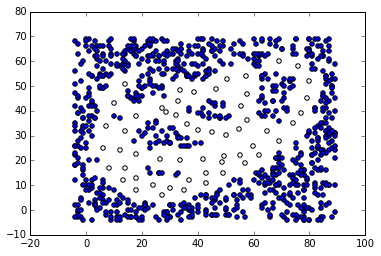
\includegraphics[width=\textwidth]{resources/Background/svs_samples} 
        \caption{Sampled Positive(white) and Negative(blue) Points}
        \label{fig:svs1}
    \end{subfigure}
    \hfill
    \begin{subfigure}[b]{0.4\linewidth}
        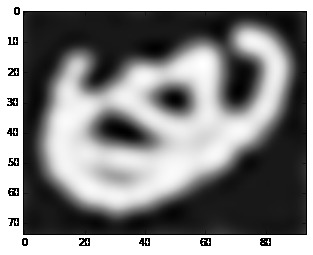
\includegraphics[width=\textwidth]{resources/Background/trained_svs} 
        \caption{Trained SVS Shape}
        \label{fig:svs2}
    \end{subfigure}
    \caption{SVS Training Points and Trained Shape}
\end{figure}

Figure \ref{fig:svs1} shows the training points where blue and white are marked as negative and positive respectively. Figure \ref{fig:svs2} revealed the final trained SVS plot, in which write colour means points are considered as part of shape with high possibility while black colour means the opposite.

\subsection{SVS Feature Points}
With SVS shape representation, reliable scale, rotation and translation invariant feature points can be retrieved based on decision function \ref{eq:svs}. Four types of feature points are produced by SVS representation: gradient based, support vector based, curvature based and entropy based feature points.

\subsubsection{Gradient Based Feature}
The gradient feature is reliable because gradient orientation is stable while gradient magnitude differs by constant factors. Gradient can be found by finding first derivative of $f(x)$ \cite{Nguyen2013}:
\begin{equation}
\label{eq:svsgrad}
\nabla f(x)=2\gamma\sum^m_{i=1}\alpha_iexp(-\gamma||x-x^*_i||^2)(x^*_i-x)
\end{equation}
where gradient orientation given by $\frac{\nabla f(X)}{||\nabla f(X)||}$. Experiments in \cite{Nguyen2013} shows gradient is stable for higher gradient magnitude points.

\subsubsection{Support Vector Based Feature}
Support vectors are claimed suitable to be feature points on it selves, due to their discriminative power of training decision function and gradient. But support vectors are sensitive to object shape. Shape deformation affects support vectors significantly.

\subsubsection{Curvature Based Feature}
Curvature based features tend to calculate points with sharp curves on decision function. Especially for 2D situation, eigenvalues of Hessian matrix is close related to curvature value:
\begin{equation}
\label{eq:svshessian}
H=
\begin{bmatrix}
    \frac{\partial^2f}{\partial x^2_1} & \frac{\partial^2f}{\partial x_1\partial x_2}\\
    \frac{\partial^2f}{\partial x_1\partial x_2} & \frac{\partial^2f}{\partial x^2_2}
\end{bmatrix}
=Q
\begin{bmatrix}
    \lambda_1 & 0\\
    0 & \lambda_2
\end{bmatrix}
Q^{-1}
\end{equation}
where points $(x_1,x_2)$ having large curvature associated with large eigenvalue in both dimension. Curvature features are highly discriminative but is not appropriate for shape matching.

\subsubsection{Entropy Based Feature}
Another similar measurement for selecting feature points is using entropy of local gradient orientation. The entropy is computed as \cite{Nguyen2013}:
\begin{equation}
\label{eq:svsentropy}
-\sum_{i=1}^np_i\log_2(p_i)
\end{equation}
where $p_i$ is the weight of bin $i$ and $n$ is number of bins in histogram. High entropy is proportional to gradient directional variation. The feature also provides highly reliable descriptor but are difficult to compute in higher dimension.
\section{Optical Flow}
\label{sec:bg_opticalflow}
Optical Flow is the motion of objects revealed in image sequences or videos \cite{fleet2006optical},\cite{Sun2010}. By estimating optical flow between frames in video sequences, motion, translation, deformation and many feature can be revealed. Optical flow is applicable under specific assumptions:
\begin{itemize}
  \item Motion of objects is smooth and gradually over time.
  \item Illumination is relatively consistent in given sequence. To be more specific, the pixel measurement in a small region remain the same despite of location changes.
\end{itemize}
A flow between two consecutive frames defines pixel movement from former frame to later frame. Defining former frame as \(I_n(i,j)\) where \(i,j\) represent pixel coordinate, the later frame is defined as \(I_{n+1}(i+u_{i,j},j+v_{i,j})\) where \(u_{i,j},v_{i,j}\) are horizontal and vertical translation of pixel (\(i,j\)). The fundamental algorithm of optimal optic flow is find a set of $u, v$ (flow directions) that minimised the objective error function:
\begin{equation}
E(p)=\sum^f_{n=1}\sum^{p}_{i,j\in p}[I_n(i,j)-I_{n+1}(i+u_{i,j},j+v_{i,j})]+regularisation
\end{equation}
where $f$ is number of frames in target sequence, $p$ is set of pixels in frame. Generally the error function contains a regularization term to prevent over fitting. Recent researches also suggest appending subspace constrains to error function \cite{Garg2013, Garg, Garg2013a}. 

\begin{figure}[h]
\centering
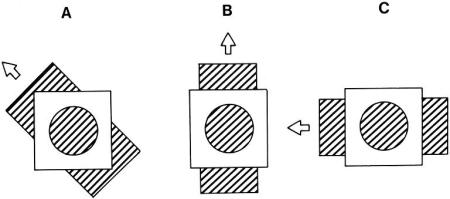
\includegraphics[width=0.9\textwidth]{resources/Background/aperture_problem}
\caption{Aperture Problem}
\label{fig:aperture_problem}
\end{figure}

\subsection{Aperture Problem}

Optical flow suffers from Aperture Problem. the aperture problem occur when determine global motion of objects from a small fraction of observation field. Figure \ref{fig:aperture_problem} demonstrate a situation when aperture problem occurs. Squares A, B and C all having different motion direction. But from only the circle observation field, objects are all classified as moving towards top left.

% Optical Flow is the motion of objects revealed in image sequences or videos \cite{fleet2006optical},\cite{Sun2010}. A flow between two consecutive frames is how pixels moves from former frame to later one. If we define former frame as \(I_1(i,j)\) where \(i,j\) represent pixel index, the later frame can defined as \(I_2(i+u_{i,j},j+v_{i,j})\) where \(u_{i,j},v_{i,j}\) are horizontal and vertical flow direction of pixel (\(i,j\)). An optimal optic flow is the set of $u, v$ (flow directions) that minimised the objective function \(\sum[I_1(i,j)-I_2(i+u_{i,j},j+v_{i,j})]\).

% In our situation, we use the idea of optical flow and apply on set of images so the flow direction should represent the correlation between objects in this case ears. Our Target is to build deformable models based on flows with an extension of deformation field where each deformed shapes are correlated. We build a flow between objects and try to minimising the following objective functions in terms of p and v.

% \begin{equation} ||I^t_p-I^{t-1}_p|| + ||U-Av||_f^2 + \sum[TV(Av)] + v.L.v^T\end{equation}

% Where \(p\) is an optimal parameter that miminise the difference between consecutive frames. \(U\) is the supervising data flow and A is eigenflow matrix with corresponding weight parameter v. The term \(\sum[TV(Av)]\) is the total variation and \(v.L.v(T)\) is used to smooth the changing between consecutive frames.
\section{Supervised Descent Methods (SDM)}
\label{sec:SSD}
As section \ref{sec:bg_aam} briefly discussed, Newton's descent method played an important role in optimising non-linear cost functions. It is widely used as the second order descent methods approach are considered robust, fast and reliable for nonlinear optimization~\cite{Xiong2013}. However few major disadvantages affect second order descent methods: (1) Function might not be analytical differentiable. (2) Hessian might be computational intensive to calculate. (3) Hessian might not be positive semidefinite, in other word the function might not be convex. (4) Functions required to be twice-differentiable.

Supervised Descent Method (SDM) are used to replace Gauss-Newton optimization. SDM proposed the idea that descent method directions can be supervisory trained, which leads to significantly reduce in computational cost since calculation of Jacobian, especially Hessian matrices is avoid. In training phase, supervised descent method learns a set of descent directions that minimise mean of nonlinear least square error functions at sampled points. In testing phase, the error function are optimised with pre-trained descent directions without computing Jacobian or Hessian.

% \begin{figure}[t]
% \centering
% \includegraphics[width=0.8\textwidth]{figures/SDM_Overview.png}
% \caption{Training procedure of SDM.}
% \label{fig:smd_training}
% \end{figure}

\subsection{SDM Algorithms}
\label{sec:SDMs}
For any given image $d \in R^{m}$ having $m$ pixels with corresponding $p$ landmarks $d(x) \in R^{p}$, feature extracted image at lanmark points is defined as $h(d(x)) \in R^{128p}$. Features e.g. Histograms of Oriented Gradients (HoGs) and Scale Invariant Feature Transform (SIFT)~\cite{Dalal2005,SIFT} are chosen due to they are robust representations agains noise arnd artifacts. Generally, an image alignment algorithm are defined~\cite{Xiong2013}:
\begin{equation}
\label{eq:ssdnd}
f(x_{k+1})=||h(d(x_k+\delta x))-\Phi_*||^2_2
\end{equation}
where at initialisation $x_0$ represents initial representation of landmarks which generated by simple object detector, $x_*$ is ground truth manual annotated landmarks, $x_k$ will be updated at the end of each iteration by $x_k+1=x_k + \delta x$ and $\Phi_* = h(d(x_*))$ represent feature extracted training image. 

However, with Newton's descent methods, calculate $\delta x$ requires computation of Jacobian and Hessian. A Taylor expansion of equation \ref{eq:ssdnd} are:
\begin{equation}
\label{eq:ssdndtaylor}
f(x_{k+1})=f(x_k)+J_f(x_k)^T\delta x+\frac{1}{2}\delta x^TH(x_k)\delta x
\end{equation}
where Jacobian $J_f{x_k}$ and Hessian $H(x_k)$ matrix are of $f$ evaluated at $x_k$. $\delta x_k$ has closed-form solution:
\begin{align}
\label{eq:ssddx}
R_{k+1}=\delta x_{k+1} = -H^{-1}J_f = -2H_{-1}J^T_h(\delta \Phi_k) \\
x_{k+1}=x_k+\delta x_k = x_{k}-2H_{-1}J^T_h(\delta \Phi_k)
\end{align}
where $J_f$ can be shown equivalent as $J^T_h(\delta \Phi_k)$, $\Phi_k=\Phi_k-\Phi_*$, $\Phi_k=h(d(x_k))$ and $R_k$ is referred as descent direction. In the above solution, $\Phi$ needs to be twice-differentiable means feature extractor $h$ has to have $2^{nd}$ order derivative, which is normally achieved with numerical approximation that generally involves heavy computation.

Supervised Descent Method introduces methods to train descent directions $R_k$ to avoid evaluating Jacobian and Hessian thus improves performance and removes criteria of functions are twice-differentiable. With SDM, equation \ref{eq:ssddx} is rewritten as:
\begin{align}
\label{eq:ssdrx}
R_{k+1}=\delta x_{k+1} = R_k\Phi_k + b_k \\
x_{k+1}=x_k+\delta x_k = x_{k}+R_k\Phi_k + b_k
\end{align}
where SDM learns a sequence of $[R_0,\dotsc,R_k,\dotsc]$ and $[b_0,\dotsc,b_k,\dotsc]$ so the iterative computation of $x_k$ converges to $x_*$.

\subsection{SDM Training}
Suppose training images and corresponding ground-truth landmarks are defined as $[d^1,\dotsc,d^i,\dotsc]$ and $[x^1_*,\dotsc,x^i_*,\dotsc]$ correspondingly. For each training image $d^i$, initial estimation of landmarks $x^i_0$ are predicted based on optimal landmark positions and related $R_0$ and $b_0$ can be obtain from optimising cost function from multiple $x^i_0$ and $x^i_*$. The sub-sequential $R_k$ and $b_k$ can be calculated as linear regression problem:
\begin{equation}
\operatorname*{arg\,min}_{R_k,b_k}\sum_{d^i}\sum_{x^i_k}||\delta x^{ki}_*-R_k\Phi^i_k-b_k||^2
\end{equation}
where $\delta x^{ki}_*=x^i_*-x^i_k$ that is used to update $x^{^i_k}$ and $\Phi^i_k$ for next iteration. Thus the program generates sequence of $[d^1,\dotsc,d^i,\dotsc]$ and $[x^1_*,\dotsc,x^i_*,\dotsc]$ for fitting without considering Jacobian and Hessian.